\chapter{Attitude Controller Test Setup}\label{app:AttitudeControllerTest} 

\subsubsection{Setup}
\begin{figure}[H]
	\centering
	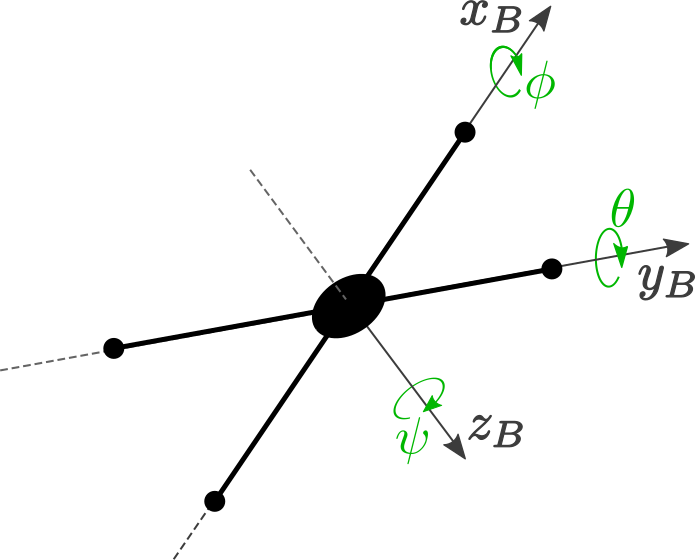
\includegraphics[scale=0.4]{figures/plusConfiguration}
	\caption{The test setup utilized to test the attitude controller.}
	\label{fig:AttitudeControllerTestsetup}
\end{figure}

\subsubsection{List of Equipment}
\begin{table}[H]
    \centering
	\begin{tabular}{|l|l|p{4.3cm}|}
		\hline%------------------------------------------------------------------------------------------------------------
		\textbf{Instrument}   &  \textbf{AAU-no.}  &  \textbf{Type}                       \\
		\hline%------------------------------------------------------------------------------------------------------------
		Quadcopter    	&  N/A 						&  (see \autoref{cha:Systemdescription}) 		      	 \\
		\hline%------------------------------------------------------------------------------------------------------------
	    Vicon System 			& 75459                 &  (see \autoref{cha:Systemdescription})                  \\
		\hline%------------------------------------------------------------------------------------------------------------
		Computer with Matlab       &  A6703		 & N/A     \\
		\hline%------------------------------------------------------------------------------------------------------------
		Attitude quadcopter holder      &  N/A		 & N/A     \\
		\hline%------------------------------------------------------------------------------------------------------------
		Attitude quadcopter connector    &  N/A		 & N/A     \\
		\hline%------------------------------------------------------------------------------------------------------------
	\end{tabular}
\end{table}


These differences may come from the test setup itself as it distorts the moments of inertia around the different axes and the location of the center of rotation with respect to the center of mass. %Furthermore, certain aspects of the behavior of the quadcopter have not been taken into account.
